\chapter{Numerics}

Ice-sheet models (ISM) essentially focus in modelling the change in mass from snow fall and snow melt onto the glacier (the glacier’s mass balance). This is usually calculated through degree day or energy balance models. ISMs must compute the flow of ice downslope under its own weight\cite{WinNT}. 

Whole-ice-sheet modelling of the Antarctic Ice Sheet (AIS) involves simulation of surface mass
fluxes (snowfall, wind drift, sublimation,melting followed by run off or refreezing), sinking or rising of the underlying bedrock in response to changing ice load heat transfer under the ice and into the bedrock affecting melting/frozen regions and the deformation rate of ice, interactions of ice shelves with the ocean and more\cite{Huybrechts_2007}

crucial input data such as bed elevation,surface elevation, and ice thickness\cite{Huybrechts_2007}


% The base of the ice sheet is buried beneath kilometres of ice, so measuring it in great detail is almost impossible.  Therefore, we have to make certain simplifications to the equations and group together physical properties in model ‘parameters’ which represent the conditions at the base of the ice sheet.


% SSA ignores vertical shear, limiting accuracy near grounding lines.

% The following are examples of variables used in models
% Known inputs:
% \begin{itemize}
%     \item Temperature data
%     \item Precipitation data
%     \item Annual temperature range
%     \item Sea level
%     \item Sea surface temperature
%     \item P/T lapse rate
%     \item Geothermal heat flux
% \end{itemize}
% Model constants:
% \begin{itemize}
%     \item Ice density
%     \item Sea water density
%     \item Gravitational acceleration
%     \item Sliding exponent
%     \item Density of mantle
%     \item Thermal conductivity of ice
% \end{itemize}
% Tuned parameters (dynamic calibration)
% \begin{itemize}
%     \item Degree day factors snow/ice
%     \item Sliding exponent
%     \item Calving rate coefficient
%     \item Deformation coefficient
%     \item Refreezing
% \end{itemize}
% To match observations
% \begin{itemize}
%     \item Observed Glacier length
%     \item Observed Glacier Geometry
%     \item Observed Glacier volume
%     \item Observed Glacier velocity
% \end{itemize}


\begin{Figure}
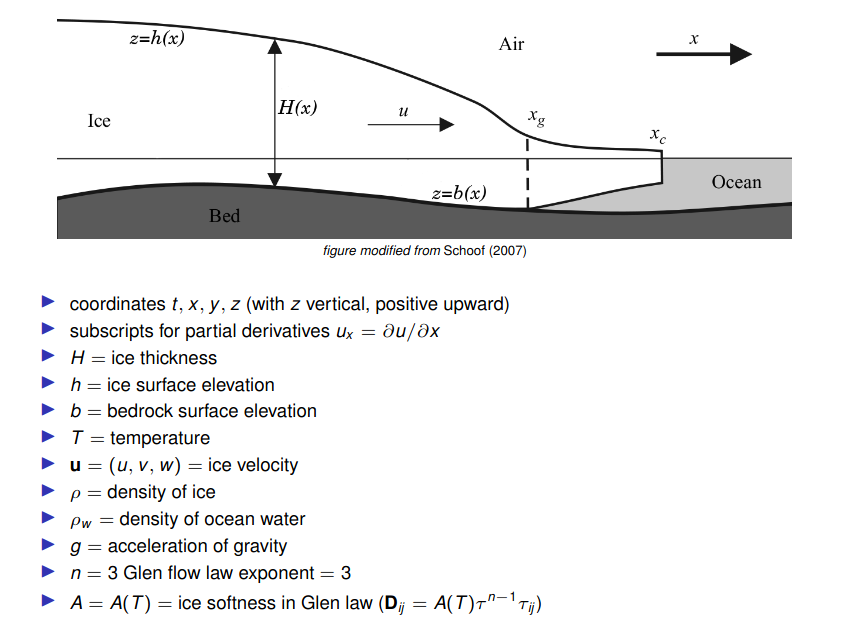
\includegraphics[width=0.9\linewidth]{numerical_modelling_of_glaciers.png}
\captionof{figure}{figure taken from\cite{modelling_ppt}}
\label{fig:parameters}
\end{Figure}

\section{ISSM: Continental-Scale Ice Sheet Modelling}
The Ice Sheet System Model (ISSM) was developed and is used for simulating ice sheet flow at continental scales. ISSM, a finite element, thermomechanical model, incorporates high-order stresses and high spatial resolution capabilities\cite{ISSM}. The Larour et al. (2012) ISSM paper discusses the different ice flow models within the software, including the full-Stokes, Blatter-Pattyn, Shallow-Shelf, and Shallow Ice Approximations, highlighting their individual strengths and limitations. It also explores numerical methods employed, such as static adaptive mesh refinement and inverse methods for parameter estimation. Finally, the study showcases the application of ISSM to the Greenland Ice Sheet, demonstrating its capacity to model the ice flow velocity with high accuracy, using data assimilation techniques to infer the basal drag coefficient.

    % ISSM offers SIA, SSA, BP, and FS formulations, allowing for different levels of complexity and computational efficiency.

    % anisotropic adaptive mesh refinement: concentrates elements in dynamic regions like fast-flowing outlets, optimizing computational resources while preserving accuracy.

    % Data assimilation incorporates observations (e.g., surface velocity) to constrain model parameters and improve realism.

    % the BAsal drag coefficient governs basal friction, a key factor influencing ice flow velocity and the response to changes in temperature or basal conditions

    % Grounding line dynamics refer to the movement of the grounding line, impacting ice discharge and contributing to sea level rise.

    % Calving is the breaking off of icebergs, a major process of mass loss from ice sheets, influencing their size and contribution to sea level.

    % ISSM includes a thermal model with heat conduction, advection, and a penalty scheme to ensure the temperature stays below the pressure melting point.

    % Challenges include improving grounding line dynamics, incorporating calving laws, and increasing spatial resolution, requiring more efficient numerical techniques and computational power.


% Essay Questions
%     Compare and contrast the four ice flow approximations (SIA, SSA, BP, and FS) implemented in ISSM, discussing their strengths, limitations, and appropriate applications.

%     Explain the process of data assimilation in ISSM, focusing on the inversion for the basal drag coefficient. Discuss the challenges and benefits of this approach.

%     Discuss the importance of accurate representation of grounding line dynamics in ice sheet models. What are the limitations of the current implementation in ISSM, and how can they be addressed in future development?

%     Describe the role of calving in ice sheet mass balance, and discuss the need to incorporate realistic calving laws in ice sheet models like ISSM.

%     Evaluate the potential of ISSM as a tool for projecting ice sheet contribution to future sea level rise. What are the key uncertainties and areas where the model can be improved?
